\section{Lemke-Howson Algorithm}

Recall by Definition~\ref{def:BR} that a strategy profile $\sigma^*$ is a MNE
if for every $i$, the strategy $\sigma^*_i$ is a best response to
$\sigma^*_{-i}$ -- that is, for every player $i$ and for every $\sigma_i \in
\Delta^{|S_i|}$ then $u_i(\sigma^*_{-i}, \sigma^*_i) \ge u_i(\sigma^*_{-i},
\sigma_i)$. We have the following lemma:

\begin{lemma}
	Strategy profile $\sigma^*$ is a Mixed Nash Equilibrium iff for each $i$,
	each pure strategy of $i$ is either a best response to $\sigma^*_{-i}$ or
	played with probability 0.
\end{lemma}

The Lemke-Howson algorithm computes Nash Equilibria. We start by drawing the
best response diagrams, yielding polyhedra, then convert these to polytopes by
connecting all lines that go to infinity into a single point.  Then we label
each edge of this polytope with a strategy if that strategy is either a best
response, or if it is played with probability 0. A Nash Equilibrium is
represented by a fully-labelled (i.e. all pure strategies appear as labels)
pair of points in the polytopes. See Fig.~\ref{fig:polytopes} for an example in
a two-player $3\times3$ game.

\begin{figure}[h]
	\centering
	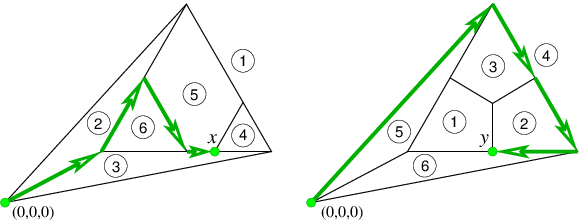
\includegraphics[width=.8\textwidth]{polytopes.png}
	\caption{A run of the Lemke-Howson algorithm}
	\label{fig:polytopes}
\end{figure}

The Lemke-Howson algorithm works by iterating over these two polytopes to find
a pair of fully-labelled vertices. As the number of strategies grows, however,
the number of points on the polytopes grows exponentially.

The procedure is:

\begin{itemize}
	\item Start at a fully-labelled point e.g. $x_1 = \ldots = x_{|S_i|} = 0$.
	\item ``Drop'' a label by traversing an edge in the diagram (this will
		``gain'' another label)
	\item Repeat step 2 until we are at another pair of fully-labelled vertices
\end{itemize}

If the input game is non-degenerate, the the Lemke-Howson algorithm finds at
least one Nash Equilibrium because:

\begin{itemize}
	\item there are finitely many vertices
	\item for a fixed label, the starting edge is unique
	\item for a fixed label, there is a unique continuation from that point
\end{itemize}

Hence we cannot visit any vertex twice.

\subsection{Slack Variables}

We can introduce variables into the constraints to turn the inequalities into
equalities, so that we are only left with non-negativity constraints. Consider
the following game:

\begin{center}
	\begin{tabular}{|c|c|c|}
		\hline
		\textbf{I}, \textbf{II} & 4 & 5 \\ \hline
		1 & 3, 1 & 3, 0 \\ \hline
		2 & 2, 0 & 5, 2 \\ \hline
		3 & 0, 4 & 6, 3 \\ \hline
	\end{tabular}
\end{center}

We get the following polyhedron for player II:

\begin{equation*}
	\begin{split}
		H_\text{II} = \{ (y_4, y_5, v) \, | \, 3y_4 + 3y_5 & \le v \\
		2y_4 + 5y_5 & \le v \\
		6y_5 & \le v \\
		y_4 + y_5 & = 1 \\
		y_4, y_5 & \ge 0 \}
	\end{split}
\end{equation*}

Let's convert this polyhedron to a polytope by dividing each inequality by $v$:

\begin{alignat}{2}
	Q_\text{II} & = \{ y \, | \, \vect{A}y \le 1, y \ge 0 \} \\
	& = \{ (y_4, y_5) \, | \, 3y_4 + 3y_5 & \le 1 \\
	& 2y_4 + 5y_5 & \le 1 \\
	& 6y_5 & \le 1 \\
	& y_4 + y_5 & = 1 \\
	& y_4, y_5 & \ge 0 \}
\end{alignat}

Now introduce new variables $x_1, x_2, x_3$ to turn each inequality into an
equality:

\begin{equation*}
	\begin{split}
		x_1 + 3y_4 + 3y_5 & = 1 \\
		x_2 + 2y_4 + 5y_5 & = 1 \\
		x_3 + 6y_5 & = 1 \\
		x_1, x_2, x_3, y_4, y_5 & \ge 0
	\end{split}
\end{equation*}

These new variables measure the distance of a point within the polytope to the
matching facet\footnote{The facets of an $n$-polytope are the faces of the
polytope with dimension $n-1$. For example, a 3-dimensional cube's facets are
its square faces, but also has 1-dimensional (edges), and 0-dimensional
(points) faces.}. A vertex in the polytope joins two line segments, so
represents two variables being set to 0. Furthermore, variable $i$ is set to 0
if and only if label $i$ is adjacent to the vertex. A solution to a system of
equations is called \textit{basic} if exactly two variables are zero.

\begin{fact}
	Non-degeneracy of a game implies that at most two lines cross at a point.
\end{fact}

\subsection{Dictionary Form}

A system of equations is in \textit{dictionary form} when we express each slack
variable as a function of the original variables. There is exactly one
dictionary per basic solution. In our example, this is:

\begin{equation*}
	\begin{split}
		x_1 & = 1 - 3y_4 - 3y_5 \\
		x_2 & = 1 - 2y_4 - 5y_5 \\
		x_3 & = 1 - 6y_5
	\end{split}
\end{equation*}

\subsection{Pivoting}

Imagine we are increasing the slack variable such that the equality still
holds. This corresponds to dropping that label in the polytope.  We can only
increase the variable so much before some variable on the right hand side (one
of the original variables) becomes 0. In the example above, since $y_4, y_5 \ge
0$, we can see that (ignoring $y_5$) $x_1$ limits $y_4$ to be at most
$\frac{1}{3}$, $x_2$ limits $y_4$ to be at most $\frac{1}{2}$, while $x_3$ does
not limit $y_4$.
